\chapter{Guardsmen and Pilgrims}

\begin{wrapfigure}{O}{\figwidth}
	\begin{center}
		
\includegraphics[width=\figwidth]{pics/2/1.png}
	\end{center}
\end{wrapfigure}
So last time the surviving remnants of a regiment of Imperial Guard found themselves the guests of Ordos Xenos. 
Several guardsmen were found to be harbouring Genestealer infections and were purged, but the remainder were given the opportunity to continue to serve the Imperium as soldiers of the Inquisition. 
So no shit there we were, 37 guardsmen who had just graduated the Darwin School of Veterancy, on an Inquisition ship, getting told that our lives would now consist of hanging out with just about the scariest people in the Imperium and doing whatever they told us to.

Serving in the Inquisition is not a very normal job, as in there's no way of knowing how things are going to work or what you'll have to do. 
Inquisitors have tons of leeway in how they do things, so each one runs their team in their own unique way. 
You might get an Inquisitor who likes to travel around following rumors and hanging out with Heroes of the Imperium, and it's your job to act as 'the cavalry' when they get into trouble. 
You might get an Inquisitor who is really into research, and wind up spending all your time guarding an incredibly disturbing science facility. 
You might get an Inquisitor who hangs out playing psychic nursemaid to a band of spies, and end up being used as a meat suit by your boss when he feels a personal touch is needed. 
Or you might get the Inquisitorial equivalent of a Pokemon Trainer.


\begin{wrapfigure}{O}{\figwidth}
	\begin{center}
		
\includegraphics[width=\figwidth]{pics/2/2.png}
	\end{center}
\end{wrapfigure}
Pokemon Trainer isn't the best way to put it, Pokemon Professor might be better.
Our Inquisitor collected teams from across the sector and handed them out to Interrogators who needed to get their feet wet leading a team. 
This was actually a pretty important role, not every Inquisitor has time or men to spare when an apprentice Interrogator is ready to move on, so they would get sent to our boss. 
He would set them up with a team and mission and keep an eye on how they did. 
He had a real name, but we all called him Professor Oak.

Oak had a fair number of recruitment teams that wandered around looking for fresh meat, one of which was hanging around our battle checking for genestealers and drafting guardsmen who wouldn't be missed. 
We got packed up and sent along to Oak's mobile base of operations and got put through a crash course in being an Inquisition Goon Squad.
Then we got split into squads of five or six, partnered up with a some combat-light teams, and handed out to dewy eyed Interrogators like the 40k equivalent of a bulbasaur.


\begin{wrapfigure}{O}{\figwidth}
	\begin{center}
		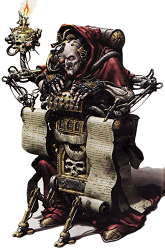
\includegraphics[width=\figwidth]{pics/2/3.png}
	\end{center}
\end{wrapfigure}
We were playing as the Guardsmen, everyone else was handled by the DM. 
Each team  was filled out to ten by other classes leaning towards the non-combat side. 
So more Adepts, Psykers, and Tech-Priests than the other classes.
There was some of everything in each group as well as the Interrogator, who could be pretty much anything. 

We worked with our DM to split our survivors up into groups, then he tacked on the sheets for our NPC associates, gave us a very vague overview of what each group's assignment was, and asked us which one we wanted to play as. 
The groups we didn't play as would all go on their own missions and the survivors would meet us when we got back to base. 
We chose the squad that was being sent as part of a two team force to check out some suspected cultist activity in a pilgrim fleet. 
Our roster consisted of five Guardsmen, two adepts, a tech-priest, a cleric, a Sister of Battle, and our Interrogator was a former Cleric.


\begin{wrapfigure}{O}{\figwidth}
	\begin{center}
		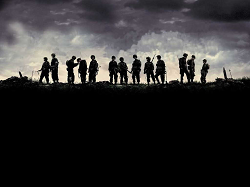
\includegraphics[width=\figwidth]{pics/2/4.png}
	\end{center}
\end{wrapfigure}
So imagine you're a guardsman that's just been recruited, fought a brutal campaign that wore down your regiment, watched the remainder of that regiment get taken out by Tyranids, then found yourself in the hands of the Inquisition. 
Then the Inquisition purges a few of your buddies, gives you an offer you can't refuse, ships you through the warp, and dumps you into a really creepy bootcamp.
Finally they split you and your remaining buddies up into squads, introduce your squad to some weird lookin guy who seems far too excited to see you, and tell you to do everything he says. 
Now you're hanging out in a bunch of passenger cabins on a navy ship going Emperor knows where with a few of your buddies, an Interrogator, three nerds (one of which is more metal than meat), a priest, and a psychotic blond bombshell wearing armor that's probably worth more than all of your squad's gear combined.
We were just a little weirded out.

Our merry band consisted of a cynic, a nervous med student, a lazy bastard, a shameless thief, and a paranoid by the names of  Sarge, Doc, Heavy, Nubby, and Twitch.
Technically the others were part of our band as well, but quite frankly we wanted nothing to do with any of them (with the possible exception of the Sister, and only in the hypothetical sense).


\begin{wrapfigure}{O}{\figwidth}
	\begin{center}
		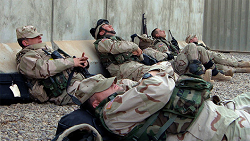
\includegraphics[width=\figwidth]{pics/2/5.png}
	\end{center}
\end{wrapfigure}
Our Interrogator and the others spent the entire journey going through the files that Oak had sent along, planning how they would hunt down the suspected cultists, sorting out who had contacts where, and brushing up on the exact flavor of the Imperial Cult that dominated the pilgrim fleet. 
We paid just enough attention to establish that we would be on ships the whole time and that we were not expected to actually do anything strenuous unless everything got screwed up. 
Then we played cards and slept a lot. 
Some people might say that two months is a long time to play cards and take naps, but those people have never served in the guard. 
And it wasn't ALL sack time, Sarge made sure we kept up on our PT and combat drill; gotta stay in shape. 
By the end of the trip we were well rested and ready to stretch our legs, whereas our teammates were wound up like springs and developing new conspiracy theories every few minutes.

We finally arrived at the Pilgrim Fleet which, as we understood it, was a bunch of ships full of hardcore zealots on their way to a world they considered holier than normal to pray, sight see, and generally replace the population that an Ork Waagh had recently removed. 
They had some sort of deal with the Ecclesiarchy to provide extra transports and fleet escorts, so it was basically just an Imperial colonization fleet, except everyone was just a teeny-tiny bit crazier than usual. 
They were hanging out in orbit around a Hive World refueling, refitting, and gathering more pilgrims. 

The Nerds and Nuts (as we called them outside of their hearing) were pretty sure that a chaos cult had infiltrated during either this stop or a previous one and was planning something very evil. 
Probably something to do with Geller Fields, or Daemons, or Plagues, or Heresy. 
We operated on the assumption that they would tell us when they figured it out. 
Anyhow our ship joined the fleet escort and a bunch of voxing and liaising started.

\begin{wrapfigure}{O}{\figwidth}
	\begin{center}
		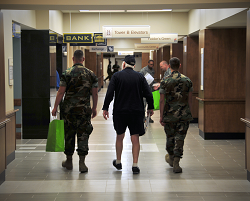
\includegraphics[width=\figwidth]{pics/2/6.png}
	\end{center}
\end{wrapfigure}
Our job was generally pretty simple; we were there to stand guard, look menacing, and always be ready to kick some ass. 
If The Boss went somewhere official we'd slap an =][= badge on and flank him like good little goons. 
If The Boss went somewhere unofficial we'd leave the badge off and slouch a little, truly we were masters of disguise. 
Whenever the Nerds and Nuts took shuttle trips to look up leads or meet contacts, at least one of us would tag along to watch their back or be on hand in case of emergency. 
Except when the Sister visited other Sororitas, we weren't invited on those trips for some reason. 

When we weren't on duty we each had our own little pastimes. 
Sarge would worry about what insanity our superiors were planning while Doc would read his beginners guide to medicine and Heavy slept. 
Nubby would wander around looking for small objects no one would miss (he did this while on duty too) and Twitch would obsessively craft tripwire traps and drink recaff. 
Twitch and Nubby didn't exactly endear themselves to the locals, but supply and perimeter defence are important parts of being a guard, so we didn't mind.

Things were going pretty well for us, no one was shooting at us, the rations were good, it didn't rain on us when we stood guard, and no one outside of our Team yelled at us to do stuff.
Occasionally we'd have to make a show of force or beat the shit out of someone who tried to mug one of our nerds, but generally things were pretty quiet.
The most excitement we had in those first few weeks was when our cleric got in a 'religious debate' and Sarge had to pistolwhip the other debater until he put down the flamer.

\begin{wrapfigure}{O}{\figwidth}
	\begin{center}
		
\includegraphics[width=\figwidth]{pics/2/7.png}
	\end{center}
\end{wrapfigure}
Eventually they must have figured something out because we all rebased to a single pilgrim ship and made ourselves the guests of the captain. 
While everyone else was running around saying things like 'The game is afoot' and 'We almost have them' and 'I can practically smell them' Sarge had us gear up and get ready for everything to go ploin-shaped. 
The cavalcade of screw-ups started with one of our nerds finding a Chaos Tome in a collection of holy relics and immediately deciding that it was his inquisitorial duty to find out exactly what flavor of Soul Destroying Evil it was. 
By reading it. 

Unfortunately  Nubby was currently on babysitting duty and was not experienced enough to know that the correct response to someone doing this to hit them until they stop being stupid. 
Instead he called for backup (which is a pretty good response in any case) while he kept the priest who owned the relic collection covered. By the time backup arrived the adept was giggling and speaking backwards.

Backup consisted of Heavy and Twitch as well as, unfortunately, the other adept and the cogboy. 
The two sane-ish nerds decided the correct response here was to try and take the book away from the gibbering adept and started chasing him around the room.
Since neither the adepts nor the tech-priest were very athletic the chase looked a lot more like a bunch of a nerdy kids trying to play tag than Inquisition agents pursuing a heretical artifact. 
None of us felt comfortable taking the initiative here, so we all just covered the doors to make sure no one entered or exited and stood there watching the demented game of keep-away. 
Then the gibbering adept finished the spell he had apparently been reciting and a minor daemon manifested.

\begin{wrapfigure}{O}{\figwidth}
	\begin{center}
		
\includegraphics[width=\figwidth]{pics/2/8.png}
	\end{center}
\end{wrapfigure}
This galvanized us nicely and all three of us started pouring las fire into the thing before it could do anything. 
Unfortunately the priest we'd been covering took the chance to run for it, then the gibbering adept followed him out the open door, then both our nerds gave chase, and now all four were running through a room full of pilgrims. 
The Priest was screaming about heretics and daemons, the adept was screaming about the Glory of Chaos, and the nerds were still trying to wrestle the book away.
The pilgrims mobbed the insane adept and tore him and the book apart in seconds, then started chasing the nerds with similar intent.

The cogboy apparently took charge and decided that not being torn to pieces was the better part of valor. 
Then he concluded that the safest place to hide from a mob of maddened imperial zealots was with the tech-priests who kept the ship running. 
The nerds ran all the way to the ships engine rooms with a steadily growing mob at their heels baying for blood. 
The tech-priests let them in and closed the door behind them, but the mob refused the disperse and settled in to siege them out.

Meanwhile the heroic guardsmen shot the minor daemon until it stopped moving, then stomped on it until it stopped being solid. 
That done we went to check on the runners and saw the mob chase them out. 
This was above our paygrade, so we decided to kick the problem upstairs and forted up while we waited for further orders. 
Eventually our Cleric and Sister arrived with Sarge and Doc in tow and The Boss voxed us all.
We gave our report, the nerds were voxed and gave theirs, then The Boss gave us our orders. 
Us guardsmen were to secure the relics and demonic remains, the Nuts were sent to talk to the pilgrims' leadership to get the mob dispersed, and The Boss would talk to the Captain and get some support sent down. 
This sounded like a pretty good plan, but by this point we'd started to suspect that we were the only competent people on the team. 
What happened next proved us right.

\begin{wrapfigure}{O}{\figwidth}
	\begin{center}
		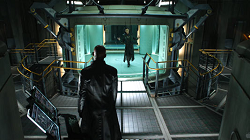
\includegraphics[width=\figwidth]{pics/2/9.png}
	\end{center}
\end{wrapfigure}
Our Interrogator marched up to the Captain of an Imperial vessel, a man who could trace his family's command of the ship back to the founding of the sector, and started giving him orders. 
This did not go over well. 
While our Interrogator was an agent of the Inquisition and had the rosette to prove it, he was NOT an Inquisitor and the Captain of an Imperial vessel is generally considered to be second only to the Emperor by their crew. 
He managed to insult the Captain in about six different ways in three sentences, which resulted in him getting his ass thrown in the brig until he remembered his manners.
The Captain then sent us a brief message instructing us to "sort out any problems with the Cargo" without bothering him or his crew. 
While we were digesting this new development the Cleric and the Sister got jumped by the cultists we'd been looking for.

Luckily the Sister and Cleric were heavily armed, incredibly paranoid, and far more level headed in an emergency than the nerds were. 
They fought a retreat to the Sororitas enclave that kept watch over this ship-load of pilgrims and dug in. 
Unfortunately the only sisters in this enclave were Hospitallers and some other non combat orders, so while they could handle a bolter they weren't suited to breaking out against the besieging cultists. 
To put it simply, they were stuck until help came, just like our adept and cogboy. 
It was down to us to pull everyone's asses out of the fire and take care of business before things got any worse.

\begin{wrapfigure}{O}{\figwidth}
	\begin{center}
		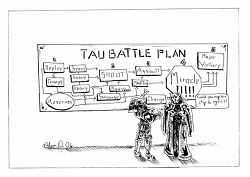
\includegraphics[width=\figwidth]{pics/2/10.png}
	\end{center}
\end{wrapfigure}
So no shit there we were, a bunch of ordinary guardsmen on a spaceship full of crazy pilgrims and cultists. 
Our boss was in the brig until the Captain was no longer pissed at him, our Nerds were trapped behind a mob that wanted to burn them as heretics, our Nuts were pinned down by a bunch of actual heretics, and it was OUR job to fix everything. 

Sarge took command of the situation and started going through the Imperial Guard NCO Disaster Response Checklist.
\todo{fix formating for list}
\begin{itemize}
	\item[Step 1:] Secure the perimeter
	\item[Step 2:] Determine chain of command
	\item[Step 3:] Call for backup if needed
	\item[Step 4:] Establish contact with friendlies
	\item[Step 5:] Combine forces with friendlies and repeat
\end{itemize}

Step 1 was already done, we had that perimeter locked down like nobodies business, there just wasn't anything we actually cared about inside of it. 
Step 2 was a bit trickier, because we were still in vox contact with the Nerds and Nuts and we didn't trust them to tie their shoes much less lead an op. 
We solved that problem by saying something about vox interference and reducing the pickup range on our combeads until we could selectively ignore them. 
Step 3 was accomplished by asking the cogboy to get his ad-mech buddies to send out the contact code for the other Interrogator team that was looking at the fleet. 
Step 4 was already done as well, we knew exactly where the friendlies were, there was just a bunch of armed cultists and an angry mob between us and them. 
All that was left was to get cracking on Step 5.

\begin{wrapfigure}{O}{\figwidth}
	\begin{center}
		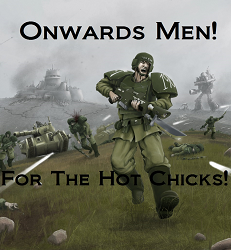
\includegraphics[width=\figwidth]{pics/2/11.png}
	\end{center}
\end{wrapfigure}
We decided that all things considered the Cleric and Sister could use our help more, and would provide more help in return, so we went for them first. 
Also they were holed up with a bunch of hot nurses as opposed to creepy machine men. 
Unfortunately we still had our orders not to let anyone touch the daemon goo or look for evil books. 
We either had to split up (which was stupid) or wait for reinforcements (which wouldn't be coming for a while) or use our initiative. 
So we tossed an incendiary grenade into the room and locked the doors and went to go rescue some hot nurses.

Unsurprisingly the cultists had set up an outer perimeter to keep out any reinforcements, so after we established where they were we fell back and started looking for other options. 
Nubby put forward the idea that the pilgrims seemed inclined to mob heretics, and these were definitely heretics, and why charge a fortified position when you can get someone else to do it for you. 
So Sarge found the nearest chapel and made a heroic speech about how the hot nuns needed our help and would probably be really grateful. 
Suddenly we had our very own mob of zealots. 

\begin{wrapfigure}{O}{\figwidth}
	\begin{center}
		
\includegraphics[width=\figwidth]{pics/2/12.png}
	\end{center}
\end{wrapfigure}
The attack went more or less perfectly. 
The mob charged in from two directions and after the cultists started mowing them down we came in from a third. 
We cut into their flank like the pros we were; suppressing, advancing, and flushing like only a squad of guardsmen can. 
When we started to hit the cultists covering the Sororitas enclave the Sister and the Cleric saw their chance and pushed forward to meet us, crushing the last of the resistance.

Unfortunately the second we rescued them the Sister and Cleric started giving orders. 
Command of the zealots was taken from us and the entire mob was redirected towards the section of ship where the cultists came from. 
Per force we tagged along, but none of us were exactly keen to be taking orders again, especially since the Sister's plan seemed to consist of "Get 'Em". 
So while the Sister and the Cleric led the mob straight into a well prepared enemy position, we appointed ourselves as the Hospitallers' guards. 
Our squad hung around at the rear of the charge and helped the saner sisters pick up the wounded while we watched for flankers and waited for the shit to hit the fan.

We fully expected the mob's suicidal rush to fail, a lightly armed force trying to press through a choke point into a fortified enemy position wasn't going to work no matter how high their morale was. 
We weren't prepared for just how hard it failed though. 
The cultists had not only set up a very nice killzone at the single entry-point to their cargo bay, they had also set up all sorts of runes and circles in the killzone. 
The wave-of-bodies attack resulted in a whole lot of people dying right on top of these runes, which immediately started glowing and doing warpy stuff. 
By the time the mob lost heart and started to retreat the cargo bay was practically filled with lesser daemons. 
We took the reverse in the flow of bodies as our cue to move forward and lay down some covering fire.

\begin{wrapfigure}{O}{\figwidth}
	\begin{center}
		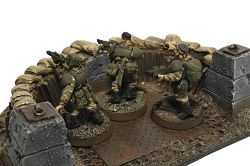
\includegraphics[width=\figwidth]{pics/2/13.png}
	\end{center}
\end{wrapfigure}
Luckily the daemons were equal-opportunity warp monsters, they spent as much time attacking each-other and the cultists as chasing down the last of our pilgrim mob and its two erstwhile leaders. 
Between the daemons' lack of coordination and our covering fire the two nutters managed to hobble most of the way back to our position. 
Most of us wanted to leave them there, but Doc sprinted out and dragged them the rest of the way to our lines and back to the Hospitallers. 
Between the two of them they had about three functional limbs and Doc spent the next few hours with the sisters patching them up.

At this point Sarge re-assumed command and decided that containment and waiting for reinforcements was the best of the available options. 
So we fell back around the corner, set up a barricade and Heavy's stubber, then settled in for the long haul. 
After a while the daemons ran out of cultists to eat and started to poke their noses around the corner and were promptly shot in the face. 
This was old hat for us really, we could defend a barricade in our sleep (literally in Heavy's case), and after a few initial rushes the daemons didn't really seem that keen on leaving their cargo bay. 
We all fell into our usual roles and routines from the guard; Twitch stared at the edge of the killzone and fired whenever he thought something might be moving while Heavy went to sleep sitting up with his eyes open and finger on the trigger. 
Behind the barricade Sarge went around yelling at people and worrying, Nubby went off to 'acquire' supplies, and Doc made eyes at one of the Hospitallers while they were both elbow deep in the Cleric's guts.

\begin{wrapfigure}{O}{\figwidth}
	\begin{center}
		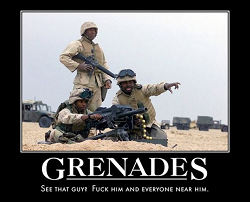
\includegraphics[width=\figwidth]{pics/2/14.png}
	\end{center}
\end{wrapfigure}
After a few hours of light trench duty, which was actually quite nice all things considered, our backup arrived. 
The second Interrogator's team (who had been doing Emperor-knows-what all this time) showed up at our barricade and Sarge explained the situation. 
Once again command was handed off, but luckily the new Interrogator decided to leave Sarge in charge of the barricade while he went to talk with the Captain and convince him not to just void our section of the ship. 
Our little troop had been reinforced to ten guardsmen, two psykers, and another damned Cleric, so Sarge decided it was time to be proactive.

Sarge wasn't happy to have another Cleric around and none us wanted anything to do with the two psykers, so the Cleric was put in charge of keeping them as far away from us as possible. 
That taken care of, a plan of attack was quickly formed and a pair of grenade launchers were scrounged up from the other teams' arsenal and Nubby's 'collection'.
We started a walking barrage up the hallway then slowly advanced our entire barricade until it was at the edge of cargo bay. 

This wasn't exactly the fastest way to clear out the daemon infestation but it was definitely the safest, not a single one of them managed to get within biting range of us. 
Once we were to the edge of the bay we just sat there and shot nades into it until we ran out, which took quite a while since Nubby could 'acquire' a surprisingly large amount of stuff. 
Eventually the launchers ran dry and it was time to clear the cargo bay the old fashion way, but the nades had done their job wonderfully. 
There wasn't really any cover left in the bay at all, so as long as we advanced slowly and carefully it was pretty easy to mow down the few remaining daemons before they got close.
All in all it went pretty well, except for the big glowing shield thing at the back of the bay.

\begin{wrapfigure}{O}{\figwidth}
	\begin{center}
		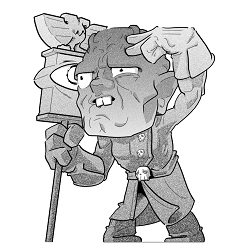
\includegraphics[width=\figwidth]{pics/2/15.png}
	\end{center}
\end{wrapfigure}
The shield was big and glowy and evil looking. 
We could sort of make out the remaining cultists inside of it doing cultisty-things, but we had no desire to get close to it. 
Quite aside from its appearance, there were quite a few corpses near it that looked like they had been turned inside-out. 
We scientifically examined the shield for a while, which is to say we shot it with every type of weapon we had sitting around, but nothing even dented it.
Eventually we gave up and Sarge voxed the replacement Interrogator and the two adepts with him for advice. 
We got a long winded explanation that included a lot of terms like "ritual entropic shield" and "drawing power directly from the warp" and "energy based daemonic lifeform" and "attempt to psychically resonate with, then overwhelm the field" which boiled down "Go get the psykers to poke at it". 
This was not the solution we were hoping for.

We had all heard stories about psykers and had encountered a few chaos witches during one of our deployments, so none of us had any desire to be near our two psykers when they attempted to crack open the shield. 
With the exception of Sarge, the Cleric, and the other squad's leader we all fell back as far as we could and got ready for a shitstorm. 
It didn't take long, within a few seconds of the psykers walking towards the shield and getting all glowy everything went wrong.
The first psyker started screaming and was suddenly surrounded by a torrential downpour of blood, then the second psyker started growing wings and horns. 
We all promptly opened fire on the possesed psyker and quickly reduced him to a thoroughly charred corpse while Sarge decked the first psyker and dragged him back to our barricade. 
Since one psyker was unconscious and the other was a pile of smoking ashes, we decided that it was probably time to figure out our own solution to the problem.

\begin{wrapfigure}{O}{\figwidth}
	\begin{center}
		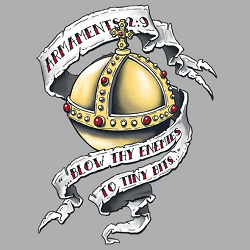
\includegraphics[width=\figwidth]{pics/2/16.png}
	\end{center}
\end{wrapfigure}
Our 'experiments' had established that las fire and grenades didn't do much to the shield, but since we were guardsmen we felt sure that enough faith and firepower could solve anything. 
We set up positions around the shield and started continuously plinking las fire into it, because when you have a fusion reactor to recharge your cells from you might as well lay down some indiscriminate suppressive fire. 
While we held the fort Nubby and the Cleric were sent to 'acquire' as many explosives, holy artifacts, and priests as possible. 
While they were out scrounging Twitch made a very good argument for setting up a blast shield. 
We voxed the cogboy and his buddies (who were STILL under siege), asked them to send down some servitors with big ol' metal shipping crates, then we built a big ass wall around the shield.

When the supply run was finished and the blast shield was in place we more or less just dumped several wheelbarrows filled with holy symbols into the the walled area along with several barrels of prometheum. 
We got a lot more of the stuff than we expected, it turns out that "we're going to use it to blow up some heretics" is a pretty persuasive argument. 
After that we got the priests to bless all the explosives we could scrounge, we weren't sure it would help but it certainly wouldn't hurt and it let them feel useful. 
We tossed the holy munitions into the blast area as well and had Twitch set up the detonators. 
Then we got as far back as we could, started a ten second timer on the explosives and ran like hell.

\begin{wrapfigure}{O}{\figwidth}
	\begin{center}
		
\includegraphics[width=\figwidth]{pics/2/17.png}
	\end{center}
\end{wrapfigure}
None of us were really sure if the 'holy shrapnel' helped at all, but when we came back there was nothing left of the cultists and their shield except a glowing puddle of molten metal and a series of dents in the walls that no amount of buffing would ever remove. 
At this point Sarge declared victory and we all went to get a snack, a nap, and a cup of recaff. 
After that was done with we decided it was about time to retrieve the rest of our team and get the hell off the ship before anyone else tried to get us all killed.

We secured The Boss from the ship's brig by turning the clean-up investigation over to the second Interrogator and promising to never bringing our boss back to the ship, ever. 
While he was escorted to the shuttle we chatted with some of the priests who helped us make our giant Holy Hand Grenade and got them to smooth things over well enough for us to get our adept and cogboy back. 
Finally we got our Sister and Cleric deposited in our shuttle's infirmary, where they would stay until we handed them off to Oak's doctors for a complete set of augmetics, then we went out and got drunk.

We enjoyed a night of drinking with our friends from the other team as well as a few of more helpful pilgrim priests and our surviving nerds. 
The high point of this was us all giving Doc shit for being hung up on one of the Hospitallers then hauling his drunk ass down to their enclave and getting him to declare his undying love for her and her "dexterous hands and perfect stitching". 
We dragged him away before he could devolve into soppy poetry, piled into our shuttle and called it a night. 
By the time we all woke back up we were docked with another navy transport and on our way back to the ISS Pokemon Center.

\begin{wrapfigure}{O}{\figwidth}
	\begin{center}
		
\includegraphics[width=\figwidth]{pics/2/18.jpg}
	\end{center}
\end{wrapfigure}
The trip back was almost exactly the same as the trip out, except we hung out with the cogboy a little more and Doc was kept busy.
The tech-priest had been damn handy working with the ship's ad-mech and handling our communications, so we were promoted him to the rank of 'cogbro' and he was welcome in our quarters. 
Doc had a pretty stressful trip, it was his job to keep the Sister and Cleric alive until they could be handed off to Oak's medical teams, but he'd never had proper medical training, just a crash course in field aid and meatball surgery. 
The ship's surgeons could have helped, but the Interrogator refused to ask the captain for their help for some reason, so Doc cracked open his medical books and did the best he could. 
They lived. 
Mostly.

When we finally got back to the Inquisitor's ship we immediately went out and found the other survivors from our regiment. 
We all swapped tales of incompetent superiors, insane teammates, horrific enemies, and intense boredom until word came down that our Interrogator was being praised for his success and would be elevated to full Inquisitor. 
Everyone had a good laugh about this and we joked about where he'd find himself imprisoned next, right up until we got word that he was looking for us with the intent to add our squad to his new retinue.

We spent the next week or so hiding with the cogbro in the bowels of the ship while all of our buddies made up wild and conflicting stories about our untimely death, reassignment to a penal legion, imprisonment by the Ordos Hereticus, induction into the Astartes, and so on. 
Eventually he left along with the surviving Adept, as well as the Sister and Cleric, both of whom had more metal in them than the average tech-priest by this point. 
We all breathed a sigh of relief and returned to our regiment's little camp.

\begin{wrapfigure}{O}{\figwidth}
	\begin{center}
		
\includegraphics[width=\figwidth]{pics/2/19.png}
	\end{center}
\end{wrapfigure}
After a few weeks of R\&R, or as close as you can get on an Inquisition battleship, a runner came down and told us we were being assigned to a new team under Interrogator such-and-such, and we were to report to our shuttle immediately. 
With a weary sigh we packed up our bags (or overloaded wheelbarrow in Nubby's case) and headed out to our transport. 
When we got to the shuttle the pilot helpfully informed us that "the Interrogator, his two assistants, and his three psykers" were already aboard. 
Twitch and Nubby both tried to run for it, but the shuttle's hatch was already closed.

Twitch and Nubby were retrieved and we all moved into the main seating area of the shuttle. 
We were greeted by our new Interrogator and introduced to our new teammates, one of whom was giggling and chewing on a seat cushion. 
As we stared in horror the Interrogator gave us a quick briefing, explaining that we had been assigned to go find out why a world hadn't been supplying psykers to the Black Ships. 
We did not have a good feeling about this.






